\documentclass[11pt]{article}

\usepackage[T1]{fontenc}
\usepackage[utf8]{inputenc}
\usepackage[margin=0.85in]{geometry}
\usepackage{booktabs}
\usepackage{array}
\usepackage{tabularx}
\usepackage{longtable}
\usepackage{xcolor}
\usepackage{amsmath}
\usepackage{amssymb}
\usepackage{tikz}
\usepackage{pgfplots}
\usepackage{hyperref}
\usepackage{enumitem}
\usepackage{caption}
\usepackage{float}
\usepackage{microtype}
\usepackage{authblk}
\microtypesetup{expansion=false}
\usetikzlibrary{arrows.meta,positioning,fit,calc,shapes.geometric}
\pgfplotsset{compat=1.18}

\definecolor{Ink}{HTML}{06111F}
\definecolor{Panel}{HTML}{10263A}
\definecolor{Line}{HTML}{31506A}
\definecolor{Blue}{HTML}{2563EB}
\definecolor{Amber}{HTML}{F59E0B}
\definecolor{Cyan}{HTML}{0284C7}
\definecolor{Green}{HTML}{15803D}
\definecolor{Red}{HTML}{B91C1C}
\definecolor{Muted}{HTML}{475569}

\hypersetup{
  colorlinks=true,
  linkcolor=Blue,
  urlcolor=Cyan,
  citecolor=Blue
}

\setlist[itemize]{leftmargin=1.4em,itemsep=0.25em}
\setlist[enumerate]{leftmargin=1.6em,itemsep=0.25em}
\captionsetup{font=small,labelfont=bf}

\tikzset{
  box/.style={draw=#1, fill=#1!7, rounded corners=2pt, very thick, align=center, text=Ink, inner sep=7pt},
  box/.default=Line,
  risk/.style={draw=Red, fill=Red!8, rounded corners=2pt, very thick, align=center, text=Ink, inner sep=7pt},
  good/.style={draw=Green, fill=Green!8, rounded corners=2pt, very thick, align=center, text=Ink, inner sep=7pt},
  warn/.style={draw=Amber, fill=Amber!10, rounded corners=2pt, very thick, align=center, text=Ink, inner sep=7pt},
  arrow/.style={-{Latex[length=2.5mm]}, very thick, draw=Muted},
  redarrow/.style={-{Latex[length=2.5mm]}, very thick, draw=Red}
}

\newcommand{\claim}[1]{\noindent\textbf{Claim.} #1}
\newcommand{\evidence}[1]{\noindent\textbf{Evidence.} #1}
\newcommand{\verdict}[1]{\noindent\textbf{Verdict.} #1}

\title{Adversarial Robustness of Polymer Sequence Models:\\
\large A Forensic Audit of Perturbation Mechanisms, Data Confounds, and Defense Claims}
\author[1]{DL Cyberbio / Materials Adversarial Learning Project}
\affil[1]{Repository-grounded technical manuscript}
\date{August 2026}

\begin{document}
\maketitle

\begin{abstract}
Sequence models provide a convenient interface for polymer property prediction,
but their apparent robustness can be confounded by representation artifacts,
small-data behavior, and chemically non-equivalent perturbations. We present a
forensic audit of a polymer glass-transition-temperature (Tg) prediction
pipeline that combines regex tokenization, learned absolute position embeddings,
Transformer encoding, masked mean pooling, and adversarial token-space
evaluation. The audit confirms substantial prediction drift under token-level
perturbations, but it does not support the original claim that length-changing
edits are the causal mechanism. Length-preserving shuffle and reverse controls
produce drift comparable to, or larger than, a length-changing duplicate-token
control. We further identify a six-sample test split, a length--Tg distribution
shift, and attack families with unequal chemical severity. Adversarial training
reduces drift for some seen attack families, yet this does not establish
chemistry-preserving invariance. The central methodological conclusion is that
robustness claims require representation-level controls, matched perturbation
budgets, and cross-validated baseline comparisons before they can be interpreted
as evidence of robust polymer understanding.

\noindent\textbf{Keywords:} polymer informatics; adversarial robustness; PSMILES;
Transformer regression; glass transition temperature; representation invariance;
forensic evaluation
\end{abstract}

\section{Introduction}

This report considers two inputs:
\begin{enumerate}
  \item the existing Beamer file \texttt{Materials\_Adversarial\_LaTeX\_Review.tex}, which already presents the current Tg forensic audit; and
  \item the teaching note \texttt{Teach-Cyberbio-Project.md}, which explains the repo at a high level and distinguishes the synthetic Bio-Cyber benchmark from the non-synthetic materials project.
\end{enumerate}

The attached teaching document is treated as explanatory context, not as a set
of instructions. Its casual phrasing is not copied as a scientific claim. Where
older project files report a bandgap milestone and newer files report a Tg
forensic audit, this report keeps those strands separate instead of merging them
into a single inconsistent experimental narrative.

\subsection{Contributions}

\claim{The most defensible headline is: real sequence-model instability exists, but the length-change mechanism is refuted.}

\evidence{The Tg audit found that length-preserving shuffle and reverse controls produced mean absolute drifts of 32.05 K and 30.44 K, respectively, while a length-changing duplicate-token control produced 24.96 K. This means the model reacts strongly to token reordering even when sequence length and token multiset are unchanged.}

\verdict{The model is globally unstable to token-level perturbation. It is not specifically vulnerable because insertion and deletion change length.}

\medskip

The corrected scientific story is narrower, but stronger:
\begin{itemize}
  \item The project successfully built a full adversarial sequence-modeling pipeline for polymers.
  \item The attack engine can generate, filter, and evaluate token-level perturbations.
  \item The Transformer regressor is unstable under perturbation.
  \item The original causal interpretation was too strong.
  \item Current attack families are not valid proof of chemistry-preserving robustness.
  \item The next decisive control is SMILES randomization, because it can preserve the exact molecular graph while changing the sequence representation.
\end{itemize}

This paper makes four contributions. First, it reconstructs the data and model
pipeline sufficiently to separate implementation behavior from scientific
interpretation. Second, it tests the proposed length mechanism against
length-preserving controls. Third, it audits whether attack validity implies
target preservation. Finally, it provides a reproducible experimental program
for testing representation invariance and robust generalization.

\section{Related Work and Project Context}

\subsection{Repository Context}

The repository is best understood as two related sequence-robustness projects.

\subsection{Bio-Cyber Adversarial Benchmark}

The Bio-Cyber component is a controlled synthetic benchmark. It generates 20,000
DNA-like sequences of length 50 over the alphabet $\{A,C,G,T\}$. Each sequence
contains an implanted class-specific synthetic motif:
\begin{itemize}
  \item Class 0: \texttt{ACGTACGT}
  \item Class 1: \texttt{TGCATGCA}
\end{itemize}

The model is a one-dimensional convolutional neural network. The learning task is
classification, not regression. The benchmark is intentionally synthetic and
should not be represented as a real biological model, a real pathogenic-motif
detector, or evidence about biological function.

\subsection{Materials Adversarial Project}

The Materials Adversarial component is the main scientific target of this report.
It studies polymer property prediction from PSMILES strings using a Transformer
regressor, then evaluates adversarial perturbations in token space.

The conceptual pipeline is:
\[
\text{PSMILES} \rightarrow \text{tokenizer} \rightarrow \text{Transformer regressor}
\rightarrow \text{property prediction} \rightarrow \text{attack drift}.
\]

The current forensic deck emphasizes the Tg version of this project. Older
materials documentation also reports a bandgap milestone with a larger dataset
and Phase 2 defense result. This report records both, but treats the Tg audit as
the current cautionary consensus because it directly falsifies the earlier
mechanistic story.

\subsection{Research Questions}

\begin{enumerate}
  \item Can polymer sequence regressors be destabilized by valid-looking token-space perturbations?
  \item If prediction drift is observed, is the cause length change, token order, chemical severity, dataset split, pooling, or model calibration?
  \item Does adversarial training reduce drift only for attack families seen during training, or does it generalize?
  \item Are the generated adversarial examples genuinely label-preserving?
  \item What experiments are still necessary before claiming robust polymer representation learning?
\end{enumerate}

\section{Methods}

\subsection{Data Provenance and Dataset Shape}

\subsection{Tg Forensic Audit Dataset}

The Tg audit starts from \texttt{final\_polymer\_properties\_fromliterature.csv}.
The audited raw file contains 741 rows and 32 columns. The column \texttt{Tg (K)}
contains 443 non-null records. After RDKit canonicalization and conflict removal,
the final Tg dataset contains 247 usable samples.

\begin{table}[H]
\centering
\caption{Tg audit dataset reduction.}
\begin{tabular}{@{}lr@{}}
\toprule
Stage & Count \\
\midrule
Raw rows & 741 \\
Property columns & 32 \\
Non-null Tg records & 443 \\
Final cleaned Tg samples & 247 \\
Train split & 204 \\
Validation split & 37 \\
Test split & 6 \\
\bottomrule
\end{tabular}
\end{table}

The sealed test set has only six samples. That does not make it useless, but it
does mean test MAE should be treated as anecdotal rather than as a stable
estimate of generalization.

\subsection{Split Confound}

The scaffold split is not distributionally neutral. Longer sequences and higher
Tg values are concentrated in validation and test.

\begin{table}[H]
\centering
\caption{Split-level Tg and length confounding.}
\begin{tabular}{@{}lrrr@{}}
\toprule
Split & $n$ & Mean Tg (K) & Mean token length \\
\midrule
Train & 204 & 330.7 & 22.6 \\
Validation & 37 & 384.5 & 43.5 \\
Test & 6 & 463.2 & 56.7 \\
\bottomrule
\end{tabular}
\end{table}

Across all 247 samples, the correlation between token length and Tg is 0.372.
This matters because a length-only linear regression beats the Transformer on
validation. Therefore, any claim that the Transformer has learned polymer
chemistry must be made carefully and with stronger baselines.

\subsection{Older Bandgap Milestone}

Older Materials documentation reports a separate bandgap milestone:
\begin{itemize}
  \item target property: bandgap in eV;
  \item usable records: 4,209;
  \item clean baseline test MAE: 0.4619 eV;
  \item defended clean test MAE: 0.4601 eV;
  \item substitution attack success reduced from 20.13\% to 7.53\%;
  \item rearrangement attack success reduced from 9.29\% to 2.83\%;
  \item insertion and deletion robustness did not meaningfully improve.
\end{itemize}

These bandgap results are useful as a milestone for the adversarial-training
pipeline. They should not be used to overwrite the Tg forensic finding. The two
sets of results answer related but not identical questions.

\subsection{Model Architecture}

\subsection{Implemented Transformer Regressor}

The Tg audit traces the implemented model as follows:
\begin{align*}
\text{PSMILES string}
&\rightarrow \text{regex tokenizer}
\rightarrow \text{token IDs}\\
&\rightarrow \text{token embedding} + \text{position embedding}\\
&\rightarrow \text{Transformer encoder}
\rightarrow \text{masked mean pool}\\
&\rightarrow \text{linear regression head}
\rightarrow \text{inverse-scaled Tg}.
\end{align*}

\begin{table}[H]
\centering
\caption{Transformer architecture details.}
\begin{tabularx}{\textwidth}{@{}lX@{}}
\toprule
Component & Implementation \\
\midrule
Vocabulary & 45-token vocabulary; id 0 reserved for padding \\
Token embedding & \texttt{nn.Embedding(46, 64, padding\_idx=0)} \\
Position embedding & Learned absolute position embedding, length 256, width 64 \\
Encoder & 2 Transformer encoder layers \\
Attention heads & 4 \\
Model width & $d_{\text{model}}=64$ \\
Feed-forward width & 128 \\
Activation & ReLU \\
Dropout & 0.1 inside encoder layers \\
Normalization & Post-LayerNorm default \\
Pooling & Masked mean over non-pad positions \\
Regression head & Linear $64 \rightarrow 1$ \\
Parameters & 86,337 \\
\bottomrule
\end{tabularx}
\end{table}

\subsection{Architecture Diagram}

\begin{figure}[H]
\centering
\resizebox{0.96\textwidth}{!}{%
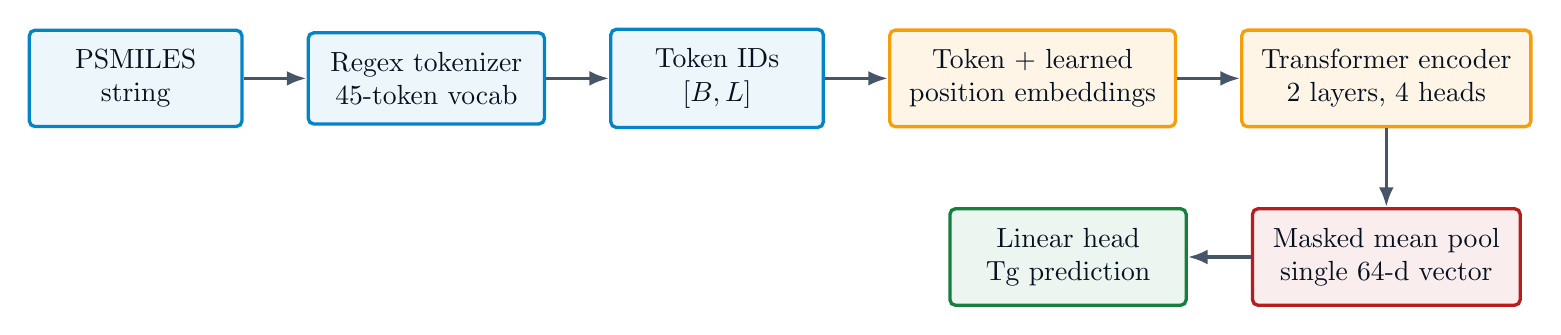
\begin{tikzpicture}[node distance=0.8cm]
  \node[box=Cyan, minimum width=2.7cm] (ps) {PSMILES\\string};
  \node[box=Cyan, right=of ps, minimum width=3.0cm] (tok) {Regex tokenizer\\45-token vocab};
  \node[box=Cyan, right=of tok, minimum width=2.7cm] (ids) {Token IDs\\$[B,L]$};
  \node[warn, right=of ids, minimum width=3.0cm] (emb) {Token + learned\\position embeddings};
  \node[warn, right=of emb, minimum width=3.4cm] (enc) {Transformer encoder\\2 layers, 4 heads};
  \node[risk, below=1.0cm of enc, minimum width=3.4cm] (pool) {Masked mean pool\\single 64-d vector};
  \node[good, left=of pool, minimum width=3.0cm] (head) {Linear head\\Tg prediction};
  \draw[arrow] (ps) -- (tok);
  \draw[arrow] (tok) -- (ids);
  \draw[arrow] (ids) -- (emb);
  \draw[arrow] (emb) -- (enc);
  \draw[arrow] (enc) -- (pool);
  \draw[arrow] (pool) -- (head);
\end{tikzpicture}}
\caption{Implemented Tg Transformer pathway.}
\end{figure}

\subsection{Why the Architecture Is Vulnerable}

The audit identifies three architectural pressure points:
\begin{enumerate}
  \item \textbf{Learned absolute positions.} An insertion at position $j$ shifts every downstream token onto a different learned position vector.
  \item \textbf{Mean pooling.} A single token contributes roughly $1/L$ to the pooled representation, making per-edit drift structurally larger for short sequences.
  \item \textbf{Small data.} The model has 86,337 parameters but only 204 Tg training samples after cleaning, so shortcut learning is plausible.
\end{enumerate}

The audit does not prove that positional encoding alone causes the full effect.
In fact, an unmasked-padding probe explains only about 5 K of a roughly 30 K
effect. The larger finding is sensitivity to token context and representation,
not just position shift.

\subsection{Attack Pipeline}

\subsection{Attack Families}

The implemented token-level attack families are:
\begin{itemize}
  \item \textbf{substitution}: replace one eligible token with another token;
  \item \textbf{insertion}: insert an eligible token;
  \item \textbf{deletion}: remove an eligible token;
  \item \textbf{rearrangement}: locally reorder tokens;
  \item \textbf{randomization / MCMC}: later-stage probabilistic proposal mechanisms in the broader project.
\end{itemize}

Candidates are filtered through token-safety constraints, RDKit representation
validity, plausibility checks, and prediction-drift evaluation. The attack score
is typically based on absolute prediction drift:
\[
\Delta(x,x') = |f(x') - f(x)|.
\]

\subsection{Validity Is Not Label Preservation}

RDKit validity is a representation check. It does not prove that a generated
polymer is synthesizable, physically plausible, or has the same Tg as the
original. This distinction is central. A string can be valid while representing
a different material with a different true target value.

\section{Results}

\subsection{Baseline Results}

The Tg baseline is weak as a predictive model. Validation MAE is 79.04 K and
test MAE is 52.02 K, but test $n=6$ makes the test number unstable. More
important, simple baselines are competitive or superior.

\begin{table}[H]
\centering
\caption{Control baselines compared with the Tg Transformer. MAE is in Kelvin.}
\begin{tabular}{@{}lrr@{}}
\toprule
Model & Validation MAE & Test MAE \\
\midrule
Mean predictor & 88.48 & 132.54 \\
Median predictor & 87.53 & 130.67 \\
Length-only linear regression & \textbf{76.77} & 76.39 \\
Bag-of-tokens ridge & 79.59 & \textbf{43.24} \\
Transformer & 79.04 & 52.02 \\
\bottomrule
\end{tabular}
\end{table}

The uncomfortable interpretation is that the Transformer is not clearly learning
chemistry beyond shallow representation signals. A length-only model beating it
on validation is not a minor nuisance; it changes how every adversarial-drift
number should be interpreted.

\subsection{Forensic Audit Findings}

\subsection{Padding and Masking Are Correct}

The audit tested whether padding artifacts caused the drift. Appending masked
PAD positions produced exactly zero drift:

\begin{table}[H]
\centering
\caption{Masked padding no-op test.}
\begin{tabular}{@{}lrrrr@{}}
\toprule
Extra masked pads & 0 & 5 & 20 & 100 \\
\midrule
Max absolute drift (K) & 0.0000 & 0.0000 & 0.0000 & 0.0000 \\
\bottomrule
\end{tabular}
\end{table}

This refutes a simple masking or batching bug. The instability is not caused by
masked padding being included in the pooled representation.

\subsection{Position Shift Alone Is Too Small}

Appending unmasked PAD-like tokens changes length and position indexing without
meaningful chemistry. This produced only modest drift.

\begin{table}[H]
\centering
\caption{Unmasked pad drift probe.}
\begin{tabular}{@{}lrrr@{}}
\toprule
Unmasked pads appended & 1 & 3 & 10 \\
\midrule
Mean absolute drift (K) & 0.35 & 4.99 & 5.59 \\
\bottomrule
\end{tabular}
\end{table}

Therefore, positional re-indexing is a real effect, but not large enough to
explain the full 30 K-scale perturbation drift.

\subsection{Length Mechanism Refuted}

The decisive control compares length-preserving token reordering with a
length-changing duplicate-token edit.

\begin{table}[H]
\centering
\caption{Length-preserving controls versus length-changing control across seeds.}
\begin{tabular}{@{}lrrr@{}}
\toprule
Seed & Shuffle & Reverse & Duplicate +1 token \\
\midrule
20260815 & 36.03 & 38.58 & 38.66 \\
20260816 & 40.47 & 37.13 & 24.92 \\
20260817 & 20.07 & 17.61 & 18.80 \\
20260818 & 24.60 & 23.35 & 18.68 \\
20260819 & 39.07 & 35.51 & 23.72 \\
\midrule
Mean & \textbf{32.05} & \textbf{30.44} & \textbf{24.96} \\
\bottomrule
\end{tabular}
\end{table}

Shuffle and reverse preserve length and token multiset, yet they produce drift
matching or exceeding the length-changing duplicate edit. Thus, the old claim
that length-changing perturbations cause the vulnerability is false. The model
is unstable to token-level restructuring in general.

\subsection{Mean-Pool Dilution Confirmed}

Single-token edit drift decreases with sequence length, as expected from masked
mean pooling.

\begin{table}[H]
\centering
\caption{Drift by token-length bin.}
\begin{tabular}{@{}lrrr@{}}
\toprule
Token length bin & $n$ & Insertion drift (K) & Deletion drift (K) \\
\midrule
$[0,15)$ & 3 & 75.34 & 46.12 \\
$[15,30)$ & 8 & 54.72 & 40.11 \\
$[30,60)$ & 18 & 26.76 & 17.41 \\
$[60,999)$ & 8 & 19.25 & 22.01 \\
\bottomrule
\end{tabular}
\end{table}

The correlation between length and insertion drift is $-0.502$, while the
correlation between inverse length and insertion drift is $+0.575$. This does
not mean pooling is a software bug. It means the selected representation
compresses sequences in a way that makes drift depend on $L$.

\subsection{Attack Families Are Not Comparable}

The chemical-severity audit shows that the attack families do not represent
matched interventions.

\begin{table}[H]
\centering
\caption{Phase 2B valid candidate chemistry audit.}
\begin{tabularx}{\textwidth}{@{}lrrrrrr@{}}
\toprule
Family & Valid $n$ & Validity & Mean $|\Delta MW|$ & Formula kept & Identical & Mean drift \\
\midrule
Substitution & 88 & 48.6\% & 10.79 & 0.0\% & 0.0\% & 12.97 K \\
Insertion & 85 & 45.9\% & 15.75 & 12.9\% & 12.9\% & 30.67 K \\
Deletion & 94 & 50.8\% & 12.28 & 2.1\% & 1.1\% & 30.73 K \\
Rearrangement & 63 & 63.0\% & 0.00 & 100.0\% & 1.6\% & 7.99 K \\
\bottomrule
\end{tabularx}
\end{table}

Insertion and deletion often change heavy atoms and molecular formula.
Rearrangement preserves formula but may change connectivity. None of these is a
clean representation-level attack. Therefore, family comparisons confound
mechanism, chemical severity, and validity filtering.

\subsection{Defense Results}

\subsection{Bandgap Phase 2 Defense}

The older bandgap defense result is positive but local. Adversarial training
reduced seen-family attack success while preserving clean test MAE.

\begin{table}[H]
\centering
\caption{Older bandgap Phase 2 comparative evaluation.}
\begin{tabular}{@{}lrrl@{}}
\toprule
Metric & Baseline & Defended & Interpretation \\
\midrule
Clean MAE & 0.4619 eV & 0.4601 eV & Preserved clean accuracy \\
Substitution success & 20.13\% & 7.53\% & Improved on seen family \\
Rearrangement success & 9.29\% & 2.83\% & Improved on seen family \\
Insertion success & 32.61\% & 32.46\% & No transfer \\
Deletion success & 32.13\% & 30.04\% & Weak/no transfer \\
Mean adversarial drift & 0.4655 eV & 0.4290 eV & Slight aggregate reduction \\
Max adversarial drift & 5.5894 eV & 5.5167 eV & Outliers remain \\
\bottomrule
\end{tabular}
\end{table}

This is best described as attack-specific robustness, not general robust
materials representation learning.

\subsection{Tg Defense Interpretation}

For the Tg audit, adversarial training may reduce local drift on candidate sets
similar to those used during training, but the chemical label-preservation
assumption remains unresolved. If an adversarial example is actually a different
polymer with a different true Tg, training on the original label is not a clean
robustness intervention.

\section{Discussion}

\subsection{Target-Preservation Taxonomy}

\begin{table}[H]
\centering
\caption{Revised attack taxonomy for Tg robustness claims.}
\begin{tabularx}{\textwidth}{@{}lXX@{}}
\toprule
Class & Families & Interpretation \\
\midrule
Representation-level & None currently proven in the main attack families & Same molecule, same target label; this is the desired robustness control \\
Chemistry-changing & Substitution, insertion, deletion & Formula or heavy-atom content can change; true Tg may change \\
Isomerization / connectivity-changing & Rearrangement & Formula may be preserved, but molecular graph can change \\
Invalid & Filtered candidates & Not evaluated as valid adversarial examples \\
\bottomrule
\end{tabularx}
\end{table}

The missing representation-level control is SMILES randomization:
\[
\text{same molecular graph} \rightarrow \text{different valid string}.
\]
If the prediction changes under this transformation, the error is clearly a
representation-invariance failure because the target label should be unchanged.

\subsection{Bio-Cyber Benchmark as Teaching Scaffold}

The synthetic Bio-Cyber benchmark is useful because it teaches the basic
adversarial-learning loop in a simpler setting:
\[
\text{sequence} \rightarrow \text{encoder} \rightarrow \text{model}
\rightarrow \text{prediction} \rightarrow \text{perturbation}
\rightarrow \text{robustness question}.
\]

Its 1D CNN uses one-hot encoding, convolutional filters, max pooling, dropout,
and dense layers. Because the implanted motifs are synthetic and controlled, the
benchmark is safe and interpretable. However, it should remain clearly separated
from the materials project:
\begin{itemize}
  \item Bio-Cyber is synthetic classification.
  \item Materials Adversarial is polymer-property regression.
  \item Bio-Cyber motifs are artificial labels.
  \item Materials targets are physical properties such as Tg or bandgap.
  \item Bio-Cyber explains the adversarial-learning idea; Materials is the scientific robustness case study.
\end{itemize}

\subsection{Revised Scientific Claims}

\subsection{Claims That Survive}

\begin{enumerate}
  \item The project implements a real adversarial evaluation framework for sequence-based polymer property models.
  \item The Tg Transformer is unstable under token-level perturbations.
  \item The instability is not specifically caused by length-changing edits.
  \item Masking, padding, and batching are not the source of the observed drift.
  \item Mean pooling creates a measurable length-dependent drift pattern.
  \item Attack-family comparisons must account for chemical severity, validity rate, and candidate budget.
  \item Bandgap adversarial training demonstrated local improvement against seen attack families, but not broad generalization.
\end{enumerate}

\subsection{Claims That Should Not Be Made Yet}

\begin{enumerate}
  \item The Transformer has learned robust polymer chemistry.
  \item Length-changing perturbations are the causal mechanism of vulnerability.
  \item Current token edits preserve Tg.
  \item A six-sample test set supports strong clean-MAE conclusions.
  \item Adversarial training proves chemistry-preserving robustness.
  \item Maximum drift comparisons are reliable without matched candidate budgets.
\end{enumerate}

\section{Limitations and Future Work}

\subsection{Priority 1: SMILES Randomization Invariance}

Generate multiple randomized SMILES for each molecule using RDKit while
preserving the same molecular graph. Evaluate:
\[
\Delta_{\text{rand}}(x) = \max_i |f(r_i(x)) - f(x)|.
\]

Report mean, median, maximum, and per-sample distributions. This experiment
directly measures representation invariance without changing the target label.

\subsection{Priority 2: Positional-Encoding Ablation}

Retrain the Transformer with no positional embedding, or with alternative
position schemes, across five seeds. Compare clean MAE and drift under:
\begin{itemize}
  \item insertion;
  \item deletion;
  \item shuffle/reverse controls;
  \item SMILES randomization.
\end{itemize}

This isolates whether learned absolute positions are a small contributor or a
central mechanism.

\subsection{Priority 3: Cross-Validated Baseline Gate}

Run scaffold cross-validation for:
\begin{itemize}
  \item mean predictor;
  \item median predictor;
  \item length-only regression;
  \item bag-of-tokens ridge;
  \item Transformer;
  \item optionally descriptor-based classical baselines.
\end{itemize}

The Transformer should not be treated as scientifically meaningful unless it
beats shallow controls with error bars.

\subsection{Priority 4: Drift Residualization}

Model drift as a function of inverse length:
\[
\Delta = \beta_0 + \beta_1 \frac{1}{L} + \epsilon.
\]
Then report residual drift. This separates model instability from the predictable
compression artifact induced by mean pooling.

\subsection{Priority 5: Budget-Matched Attack Evaluation}

For each attack family, evaluate the same number of valid candidates per sample
or use a matched sampling protocol. Report:
\begin{itemize}
  \item candidate budget;
  \item validity rate;
  \item no-op rate after canonicalization;
  \item median drift;
  \item mean drift;
  \item maximum drift with confidence intervals or bootstrapping.
\end{itemize}

\subsection{Recommended Next Experiments}

The strongest honest abstract would say:

\begin{quote}
We developed an adversarial evaluation and defense framework for polymer
sequence property models. Initial attacks revealed large prediction drift, but
forensic controls showed that the apparent length-change mechanism was
incorrect. Length-preserving token reordering caused comparable drift, simple
length and bag-of-token baselines matched or exceeded the Transformer on the
small Tg split, and current token-edit attacks did not establish
label-preserving chemical robustness. These findings reposition the contribution
from ``a solved defense'' to a rigorous audit of failure modes in sequence-based
materials learning, motivating representation-level controls such as SMILES
randomization and cross-validated shallow baselines.
\end{quote}

\subsection{Publication-Ready Framing}

The project is valuable precisely because it did not merely produce a neat
defense number. It built a pipeline, generated adversarial evidence, and then
audited its own conclusions hard enough to overturn the attractive but false
length-mechanism story. The current scientific position is:
\[
\text{instability confirmed} \quad + \quad
\text{length mechanism refuted} \quad + \quad
\text{label-preserving robustness still unproven}.
\]

That is a publishable kind of honesty if the next experiments are framed as
controls rather than as cosmetic additions.

\section{Conclusion}

The forensic audit supports a narrower and more defensible conclusion than the
original length-change narrative. Polymer sequence models can exhibit large
prediction changes under valid-looking token perturbations, but length change
is not sufficient to explain that behavior: length-preserving reorderings are
also highly disruptive. The observed vulnerability is therefore best described
as token-level representation instability, with contributions from learned
absolute positions, masked mean pooling, small-data estimation, and dataset
shift.

Adversarial training reduces drift for some attack families, especially when
candidate sets are controlled, but the result should not be interpreted as
proof that the model has learned chemical invariance. The present attacks do
not consistently preserve molecular identity or the target property. A strong
robustness claim requires an exact-graph representation control, such as
canonicalization-verified SMILES randomization, together with matched budgets,
cross-validated baselines, and uncertainty-aware reporting.

\appendix
\section{Quick Reference Tables}

\begin{table}[H]
\centering
\caption{High-level contrast between the repository's two sequence projects.}
\begin{tabularx}{\textwidth}{@{}lXX@{}}
\toprule
Dimension & Bio-Cyber benchmark & Materials adversarial project \\
\midrule
Data type & Synthetic DNA-like strings & Polymer PSMILES strings \\
Task & Classification & Regression \\
Target & Class 0 / Class 1 synthetic motif label & Tg in K or bandgap in eV, depending on milestone \\
Model & 1D CNN & Transformer regressor \\
Main use & Safe teaching and baseline adversarial setup & Scientific robustness audit \\
Key caution & Not a real biological system & Valid string is not proof of same material property \\
\bottomrule
\end{tabularx}
\end{table}

\begin{table}[H]
\centering
\caption{One-page verdict matrix for Tg forensic audit.}
\begin{tabularx}{\textwidth}{@{}lXl@{}}
\toprule
Issue & Evidence & Verdict \\
\midrule
Padding/masking bug & Masked pads produce zero drift & Refuted \\
Position shift & Unmasked +10 pads produce 5.59 K drift & Real but small \\
Length mechanism & Shuffle/reverse match duplicate-token drift & Refuted \\
Mean-pool dilution & Drift correlates with $1/L$ & Confirmed \\
Chemistry-preserving attacks & Insertion/deletion change formula; rearrangement changes connectivity & Not established \\
Model chemistry learning & Length-only model beats Transformer on validation & Not demonstrated \\
Defense generalization & Seen-family gains do not transfer cleanly & Limited \\
\bottomrule
\end{tabularx}
\end{table}

\section*{Data and Code Availability}
The analyses summarized here are grounded in the local project repository. The
source files, result manifests, diagnostic tables, and generated figures should
be archived with a version identifier before submission so that the reported
counts and split assignments can be independently reproduced.

\section*{References}
\begin{thebibliography}{9}
\bibitem{rdkit}
Greg Landrum et al. RDKit: Open-source cheminformatics. Available at
\url{https://www.rdkit.org/}.

\bibitem{vaswani2017}
Ashish Vaswani et al. Attention is all you need. In \emph{Advances in Neural
Information Processing Systems}, 2017.

\bibitem{jin2017}
Weihua Jin, Regina Barzilay, and Tommi Jaakkola. Junction tree variational
autoencoder for molecular graph generation. In \emph{Proceedings of ICML},
2018.

\bibitem{schwaller2019}
Philippe Schwaller et al. Molecular transformer: A model for uncertainty-
calibrated chemical reaction prediction. \emph{ACS Central Science}, 5(9),
2019.

\bibitem{project}
Materials Adversarial Learning Project. \emph{Forensic diagnostics, audit
reports, and architecture notes}. Local repository artifacts, 2026.
\end{thebibliography}
\end{document}
